\documentclass[14pt, a4paper]{extarticle}

%\usepackage[usenames,dvipsnames,svgnames,table]{xcolor}
\usepackage[
  a4paper, mag=1000, includefoot,
  left=3cm, right=1cm, top=2cm, bottom=2cm, headsep=1cm, footskip=1cm
]{geometry}

\usepackage{amsmath,amssymb,amsfonts}
\usepackage{mathtools}
\usepackage[cache=false,outputdir=.texpadtmp]{minted}

\usepackage{polyglossia}
\setmainlanguage{russian} 
\setotherlanguage{english}
\newfontfamily\russianfont[Script=Cyrillic]{CMU Serif}
\newfontfamily{\cyrillicfonttt}{CMU Typewriter Text}


% Macro: Absolute value
\DeclarePairedDelimiter{\abs}{\lvert}{\rvert}

\begin{document}

%-----------------------------------------
% Титульный лист
\thispagestyle{empty}

\begin{center}

\scriptsize{
Министерство образования и науки Российской Федерации

Федеральное государственное автономное образовательное учреждение высшего профессионального образования
}

\textbf{«Уральский федеральный университет}

\textbf{имени первого Президента России Б.Н. Ельцина»}

\textbf{\large Институт математики и компьютерных наук}

\textbf{\large Кафедра алгебры и дискретной математики}


\vfill
\vfill

\Large О фильтрации событий в физике высоких энергий с помощью нейросетей с инверсией градиента.

\end{center}

\vfill

\hspace*{0.4\textwidth}
\parbox{0.6\textwidth}{
\noindent
Квалификационная работа\\
на степень бакалавра наук\\
по направлению\\
«Математика, прикладная математика»\\
студента группы МТ-401\\
Киселева Антона Ивановича

\bigskip

\noindent
Научный руководитель\\
Клепинин Александр Владимирович,\\
кандидат физико-математических наук,\\
доцент кафедры алгебры и\\
дискретной математики ИМКН УрФУ
}

\vfill
\vfill

\begin{center}
Екатеринбург

2016
\end{center}

\sloppy

%-----------------------------------------
% Реферат
\newpage

\setcounter{page}{1}
\thispagestyle{empty}

\centerline{\large \textbf{Реферат}}

\bigskip
\bigskip

% TODO сократить
Глубокие нейросетевые архитектуры показывают превосходные результаты при наличии большого количества размеченных данных. В случае их отсутствия доменная адаптация помогает при наличии большого количества данных похожей природы, но имеющих смещенное распределение.
Одной из таких задач является фильтрация событий, полученных детекторами Большого Адронного коллайдера.
Для решения подобных задач была предложена новая архитектура для проведения доменной адаптации.
Ее суть заключается в создании нейросети с двумя выходами — один из них определяет класс, а другой домен.
Классифицирующие домен слои подключены к остальной сети при помощи слоя обращения градиента.
При проведении процедуры обучения при помощи метода обратного распространения ошибки этот слой негативно влияет на определение домена, таким образом нейросеть выделяет неспецифические для конкретных доменов признаки.

Целью этой работы является исследование применимости архитектуры нейросети со слоем обращения градиента в задаче детектирования распада частиц $\tau^- \rightarrow \mu^+ \mu^- \mu^-$.

В процессе работы была построена нейросеть, которая успешно обучается и выделяет признаки, позволяющие выделить сигнал, но не позволяющие по ним отделить реальные данные от синтетических.

\medskip

\noindent
Ключевые слова: доменная адаптация, глубокие нейронные сети.

\medskip 

\noindent
Объект исследования~— доменная адаптация глубоких нейронных сетей.

\medskip 

\noindent
Цель работы~— рассмотреть применение доменной адаптации нейронных сетей в задаче фильтрации событий, разработать методику применения таких сетей для создания неразличающего домены нейросетевого классификатора.

\medskip 

\noindent
Результаты работы: проведены эксперименты по применению данного вида нейросетей; изучено влияние изменения параметров классификатора на получаемый результат; сделан вывод насчет практической применимости доменной адаптации в данной задаче.

%-----------------------------------------
% Содержание
\newpage

\tableofcontents

%-----------------------------------------
% Введение
\newpage

\addtocontents{toc}{\protect{\contentsline{section}{\numberline{}{Введение}}{\thepage}}}
\section*{Введение}

В современном мире каждый день создается невероятное количество информации. С одной стороны, люди общаются друг с другом через социальные сети и создают таким образом миллионы текстов. С другой стороны, есть миллионы устройств, которые собирают данные — термометры, приборы учета, видеокамеры и прочее. Анализ этих данных является крайне популярной на сегодняшний день темой. Она актуальна как в исследовательской среде, так и среди бизнеса. 

Анализ данных требует использования различных методов машинного обучения, таких как машины опорных векторов или решающих деревьев. Для большинства из этих методов наличие \textit{большого объема} данных позволяет строить более точные модели. 

Одной из важных задач машинного обучения является задача классификации. К сожалению, для многих задач, сводящихся к задаче классификации невозможно получить достаточно большой объем данных, для получения хорошей модели. Это может быть связано как с тем, что для получения большого количества данных требуется затратить множество ресурсов, так и тем, что генерирующие их процессы случаются довольно редко. Помимо этого, может быть такая ситуация, что достоверность данных сомнительна.

Одной из таких задач является поиск лептонных распадов, не сохраняющих лептонный аромат. В Стандартной модели — общепринятой на данный момент модели физики элементарных частиц — считается, что аромат лептонов является физической характеристикой, которая сохраняется при распадах. В некоторых моделях физики элементарных частиц ароматы лептонов таким свойством не обладают. Успешное нахождение такого рода распадов откроет новые горизонты для физики элементарных частиц. Одним из таких распадов является распад $\tau^-\rightarrow\mu^+ \mu^- \mu^-$, который рассмотрен в работе. Формальное определение задачи дано в параграфе \ref{paragraph:task}.

Одной из наиболее точных моделей, использующейся в задаче классификации, является глубокая нейронная сеть. Мы описываем ее устройство в параграфе \ref{paragraph:theory}. Во многих задачах классификации применение глубоких нейронных сетей с архитектурой прямого распространения сигнала дает хорошие результаты. К сожалению, на данный момент эти задачи ограничиваются лишь такими, для которых имеется большое количество размеченных данных для обучения. В то же время, для некоторых задач с малым количеством размеченных данных возможно получить достаточный для обучения глубоких нейросетевых архитектур объем данных, распределение которого однако является смещенным относительно тех данных, для которых ожидается использование модели.

Важным примером таких задач являются задачи, для которых возможно получить множество размеченных синтетических данных, однако довольно часто их распределение будет отличным от реального. Обучение классификатора в условиях наличия смещения между тестовыми данными и данными для обучения называется доменной адаптацией.

Мы рассматриваем предложенную в \cite{ganin} архитектуру нейронной сети в параграфе \ref{paragraph:method}. Там же мы описываем реализацию этого метода на языке программирования Python.

В рамках исследования была построена нейросетевая архитектура прямого распространения сигнала, включающая в себя слой обращения градиента. Она описана в параграфе \ref{paragraph:architecture}. Было исследовано влияние различных параметров модели на получаемый в итоге результат. Результаты проведенных экспериментов описаны в параграфе \ref{paragraph:results}.

%-------------------------------------------------------
% Теория
\newpage
\section{Теоретический материал}
\label{paragraph:theory}

В этом параграфе дается формальное определение задачи классификации, а так же описывается один из методов ее решения — нейронная сеть.

\subsection{Задача классификации}
\label{class_task}

Предполагаем, что модель получает на вход объекты $x \in X$, которым соответствуют метки классов $y \in Y$. Предполагается, что $Y = {1, 2, ..., L}$ — конечное множество размера $L$. $S(x,y), T(x,y)$ — двумерные случайные величины на $X \otimes Y$ будем называть \textit{исходным} и \textit{целевым} распределениями (или \textit{доменами}) соответственно. Далее считаем что между ними существует некоторый сдвиг — они в целом схожи, но различны.

Предполагаем, что нам даны ${x_1, x_2, ..., x_N}$ — обучающая выборка, выделенная как из исходного, так и из целевого доменов.

Также нам известна бинарная переменная $d_i$, которая равна единице для объектов выборки из $S(x)$ и нулю для $T(x)$. Ее мы будем называть \textit{меткой домена}. При $d_i = 0$ нам известна метка класса $y_i$, иначе же нет. Именно ее нам необходимо предсказывать для тестовых данных.
 
Отметим существование такого явления, как \textit{переобучение}. Это явление, при котором частота ошибок на тестовой выборке выше, чем на обучающей. Оно возникает при использовании черезмерно сложных моделях. Методы борьбы с ней называются \textit{регуляризацией}.

\subsection{Устройство нейронной сети}

Перед тем, как описать устройство нейронной сети, введем понятие \textit{нейрона}. Под нейроном мы имеем в виду функцию $h_{w, b}(x): \mathbb{R}^{n} \rightarrow \mathbb{R}$:

\begin{equation*}
	h_{w, b}(x) = f(w^Tx) = f(\sum_i w_ix_i + b)
\end{equation*}
\begin{itemize}
\item $f: \mathbb{R} \rightarrow \mathbb{R} $ — функция активации нейрона;
\item $w_i \in \mathbb{R} $ — весовые коэффициенты нейрона.
\end{itemize}

Таким образом один слой в нейронной сети можно описать как функцию $h_{W, B}: R^n \rightarrow R^m$ из $m$ определенных выше функций, где $W$ — матрица весов слоя.

Нейронная сеть представляет собой сеть из нескольких слоев. Нейронные сети с архитектурой прямого распространения сигнала состоят из трех частей: входного слоя, скрытого слоя и выходного слоя.

\subsection{Обучение нейронной сети}
% Этот раздел важен тем, что метод основывается на свойствах этого алгоритма обучения и работает (наверно) лишь только для него.
Приведем краткое описание используемого далее алгоритма обучения нейронной сети — стохастического градиентного спуска.
% TODO цитата + алгоритм

\subsection{Слой Dropout}
В работе \cite{dropout} был предложен dropout-слой как средство регуляризации. Его суть заключается в следующем: во время обучения нейрон такого слоя присутствует в модели с фиксированной вероятностью $p$; во время же использования модели он присутствует всегда, однако его вес умножается на $p$.
 
\begin{center} % TODO formatting (captions)
	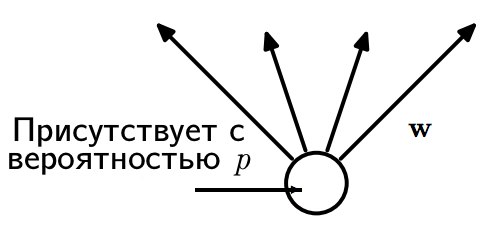
\includegraphics[scale=0.8]{images/dropout1.png}
	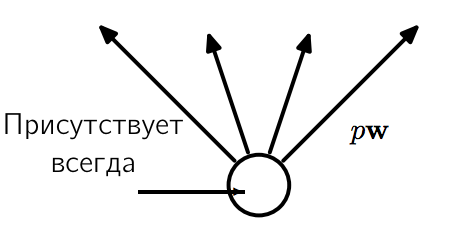
\includegraphics[scale=0.8]{images/dropout2.png}
\end{center}

\subsection{Функция активации PReLU}
В статье \cite{prelu} предлагается кусочно-линейная функция активации, под названием PReLU. Она определяется следующим образом:
\begin{equation}
	f(y_i) = \begin{cases}
		y_i, & \text{при $y_i >= 0$} \\
		a_iy_y, & \text{при $y_i < 0$}
	\end{cases}
\end{equation}
Заметим, что параметр $a_i$ уникален для каждой координаты вектора $y$. Эти коэффициенты близки к нулю и подбираются в процессе обучения. 

\begin{center}
	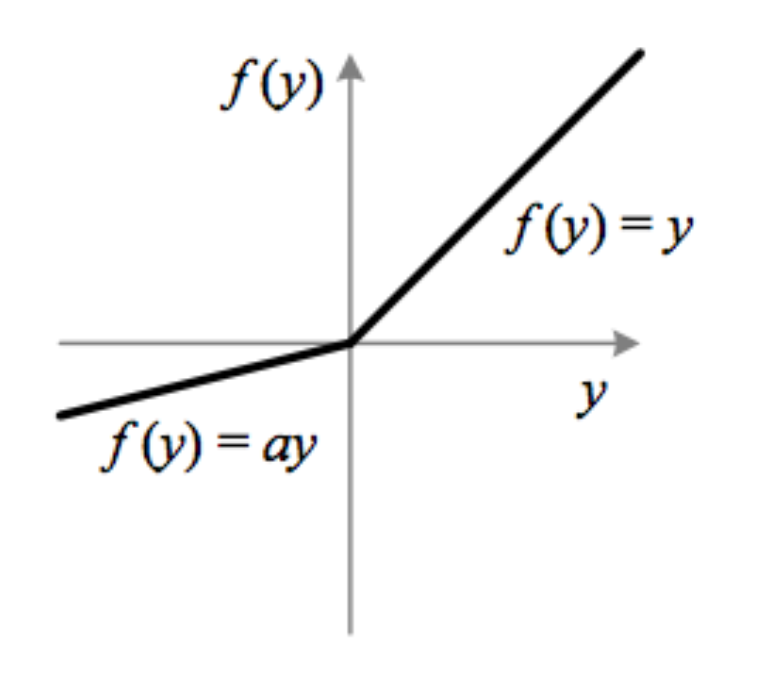
\includegraphics[scale=0.5]{images/prelu.png}
\end{center}

%-------------------------------------------------------
% Исследуемый метод
\newpage
\section{Исследуемый метод}
\label{paragraph:method}
 
Ниже мы опишем предложенную в \cite{ganin} архитектуру. Она представима в виде сети из трех отдельных сегментов.
 
Первый из сегментов будем называть \textit{экстрактором признаков} и обозначать $G_d$. Он занимается тем, что по исходному входу $x \in X$ возвращает вектор $f \in \mathbb{R}^D$. Если обозначить за $\theta_f$ параметры всех слоев экстрактора, то можно отметить что $f = G_d(x, \theta_d)$.
 
Второй сегмент $G_y$ затем продолжает первый и называется \textit{классификатором класса}. Он по выданным $G_f$ признакам $f$ возвращает метку $y$. Его параметры — $\theta_y$. Другими словами, $y = G_y(f, \theta_y)$.
 
Аналогично третий сегмент $G_d$ продолжает экстрактор признаков и возвращает метку домена $d$ и имеет параметры $\theta_d$: $d = G_d(f, \theta_d)$. Его мы будем далее называть \textit{классификатором домена}.

При процедуре обучения нашей целью является проведение \textit{доменной адаптации} — получение признаков $f$, для которых распределения $S(f) = \{G_f(x; \theta_f)~|~x \sim S(x) \}$ и $T(f) = \{G_f(x; \theta_f)~|~x \sim T(x) \}$ будут схожи. Именно с этим и справляется предложенный в \cite{ganin} метод.

Данный метод рассматривает следующий функционал:

\begin{equation}\label{E}
\begin{gathered}
E(\theta_f, \theta_y, \theta_d) = \\ \sum_{ \substack{i=1..N \\ d_i=0} }L_y(G_y(G_f(x_i; \theta_i); \theta_y), y_i) - \lambda \sum_{ i=1..N } L_d(G_d(G_f(x_i; \theta_i); \theta_d), y_i) = \\\sum_{ \substack{i=1..N \\ d_i=0} } L_y^i(\theta_f, \theta_y) - \lambda \sum_{ i=1..N }  L_d^i(\theta_f, \theta_d)
\end{gathered}
\end{equation}
\begin{itemize}
\item $L_y(·, ·)$ —~ функция потерь классификатора класса;
\item $L_d(·, ·)$ —~ функция потерь классификатора домена;
\end{itemize}

Далее, производится поиск параметров $\hat \theta_f, \hat \theta_y, \hat \theta_d$, образующих седловую точку функционала:
\begin{equation*}
	(\hat \theta_f, \hat \theta_d) = \underset{\theta_f, \theta_d}{\text{arg~min}}~E(\theta_f, \theta_y, \hat \theta_d) \\
\end{equation*}
\begin{equation*}
	\hat \theta_d = \underset{\theta_d}{\text{arg~max}}~E(\hat \theta_f, \hat \theta_y, \theta_d)
\end{equation*}

При таких параметрах с одной стороны будет достигаться минимум функции потерь для классификатора класса, а с другой максимум для функции потерь классификатора домена. Это обеспечит признаки $f$ как оптимально различающими классы, так и независимыми от домена — другими словами, произойдет доменная адаптация.

Идея метода в следующем: классификатор домена подключается к экстрактору признаков через специальный \textit{слой обращения градиента}, описанный далее. Благодаря своим свойствам, он позволяет при проведении обучения получать такие параметры $\theta_f$, которые максимизируют функцию потерь классификатора домена, но при этом такие $\theta_d$, которые ее минимизируют.

\begin{center}
	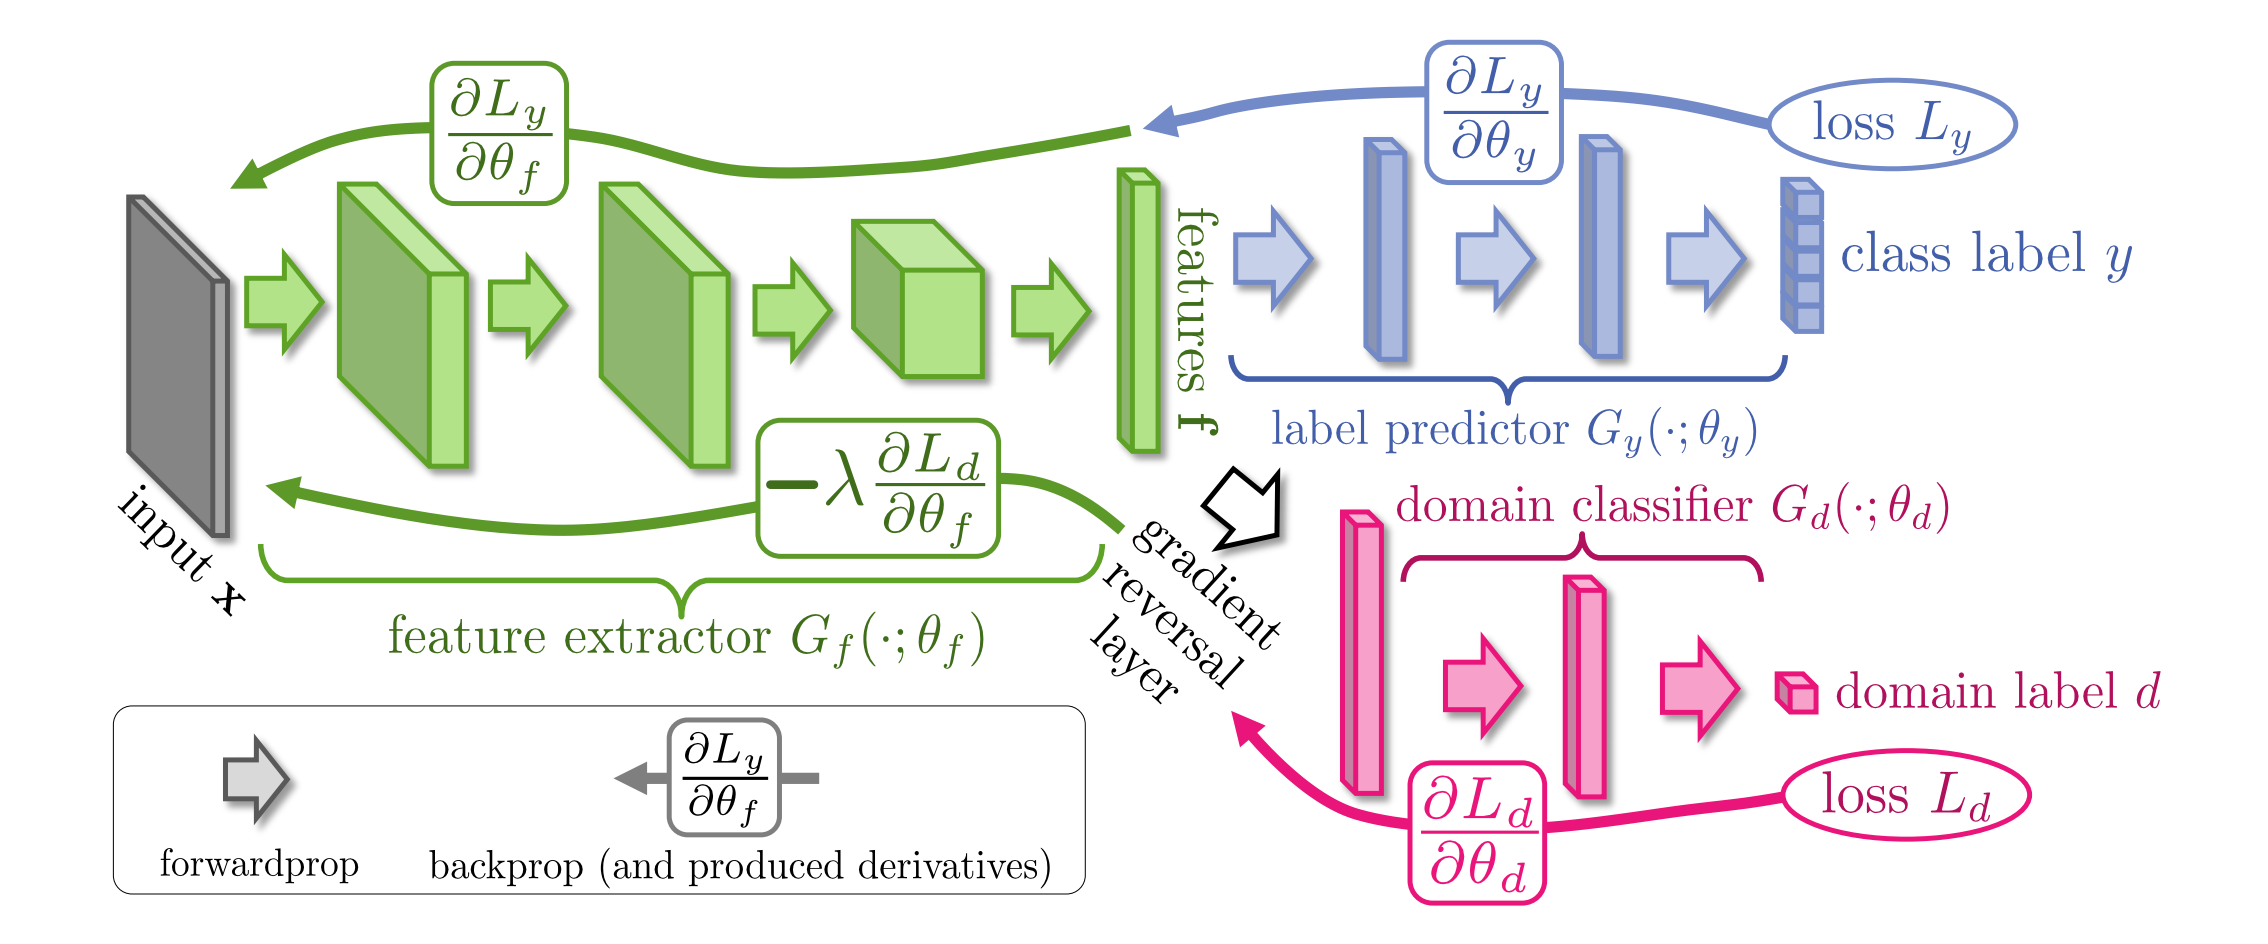
\includegraphics[scale=0.4]{images/grl_architecture.png}
\end{center}


%-------------------------------------------------------
% Задача
\newpage
\section{Задача}
\label{paragraph:task}

Для исследования метода была выбрана задача из соревнования \cite{kaggle_contest} с сайта \texttt{kaggle.com}. Оно проходило с 20 июля по 12 октября 2015 года. Соревнующимся был дан набор данных, содержащий как синтетические, так и реальные данные из эксперимента LHCb Большого Адронного Коллайдера. По этим данным было предложено построить модель, которая сможет выявлять наличие событий, соответствующих распаду $\tau \rightarrow 3\mu$. Обнаружение таких событий будет означать нарушение предсказываемого Стандартной моделью свойства сохранения аромата у лептонов, которому данный распад не подчиняется. 

Далее мы подробно опишем формат данных и использованные для ранжирования участников соревнования метрики.  

\subsection{Формат данных}
Для анализа участникам состязания были предоставлены четыре файла:
\begin{enumerate}
\item \texttt{training.csv} — набор размеченных данных для обучения классификатора, целевой переменной является переменная \texttt{signal}. Ее значение 1 описывает события сигнала, 0 — фона.
\item \texttt{check\_agreement.csv} — набор размеченных данных для проверки на согласованость (описана в \ref{agreement_metrics}). Признаки такие же, как и в \texttt{training.csv}, однако \texttt{signal} отвечает за домен — 1 для синтетических данных, 0 для реальных.
\item \texttt{check\_correlation.csv} — набор данных для проверки классификатора на коррелированность с массой. Включает дополнительный признак \texttt{mass}. Подробней описано в \ref{mass_metrics}.
\item \texttt{test.csv} — набор неразмеченных данных, для которых участникам необходимо предоставить метки классов.
\end{enumerate}

\subsection{Процедура проверки решения}

\subsubsection{Проверка на согласованность}
\label{agreement_metrics}
Так как для обучения классификатора участникам были предоставлены как реальные, так и синтетические данные, при создании хорошего классификатора возможно было бы использовать такие признаки, которые были плохо смоделированы во время получения синтетических данных. 

Чтобы избежать этого, при проверке решения используется критерий Колмогорова-Смирнова. Он рассчитывается следующим образом:
\begin{equation*}
	KS = max \abs{F_{simulation} - F_{real}}
\end{equation*}
\begin{itemize}
	\item $F_{simulation}, F_{real}$ — функции распределения для синтетических и реальных данных соответственно
\end{itemize}

Большее значение этого критерия будет означать большую зависимость между значениями классификатора на реальных и синтетических данных соответственно.
Для принятия проверочной системой решения требовалось, чтобы $KS < 0.09$.


\subsubsection{Проверка на корреляцию с массой}
\label{mass_metrics}
Помимо этого, полученный классификатор может в процессе обучения по предоставленным данным научиться восстанавливать массу исходной частицы, распад которой был зафиксирован. Такое поведение вызывает некорректную оценку фона и может привести к ложным обнаружениям сигнала. Таких обнаружений требуется избегать.

Для проверки классификатора на корреляцию с массой исходной частицы применяется критерий Крамера-Мизеса, описанный в \cite{cramer}. Для его вычисления функция распределения на всем диапазоне масс сравнивается с функцией распределения на некотором интервале. После этого итоговое значение для критерия усредняется по всем интервалам:

\begin{equation*}
	CvM_{interval} = \int (F_{global} - F_{local})^2 dF_{global},
\end{equation*}
\begin{equation*}
	CvM = <CvM_{interval}>_{interval}
\end{equation*}
\begin{itemize}
	\item $F_{global}, F_{local}$ — функции распределения для всех данных и для данных в некотором интервале масс
\end{itemize}
Чтобы решение засчитывалось, в условии задачи требуется чтобы $CvM < 0.002$.

\subsubsection{Метрика качества}
\label{quality_metrics}
Качество полученного классификатора оценивалось при помощи взвешенного показателя AUC. Этот показатель рассчитывается как площадь под ROC-кривой, построенной для результатов классификатора. В данном случае вклад в показатель AUC конкретных сегментов под ROC-кривой показан ниже:
% TODO добавить определение ROC-кривой

\begin{center}
	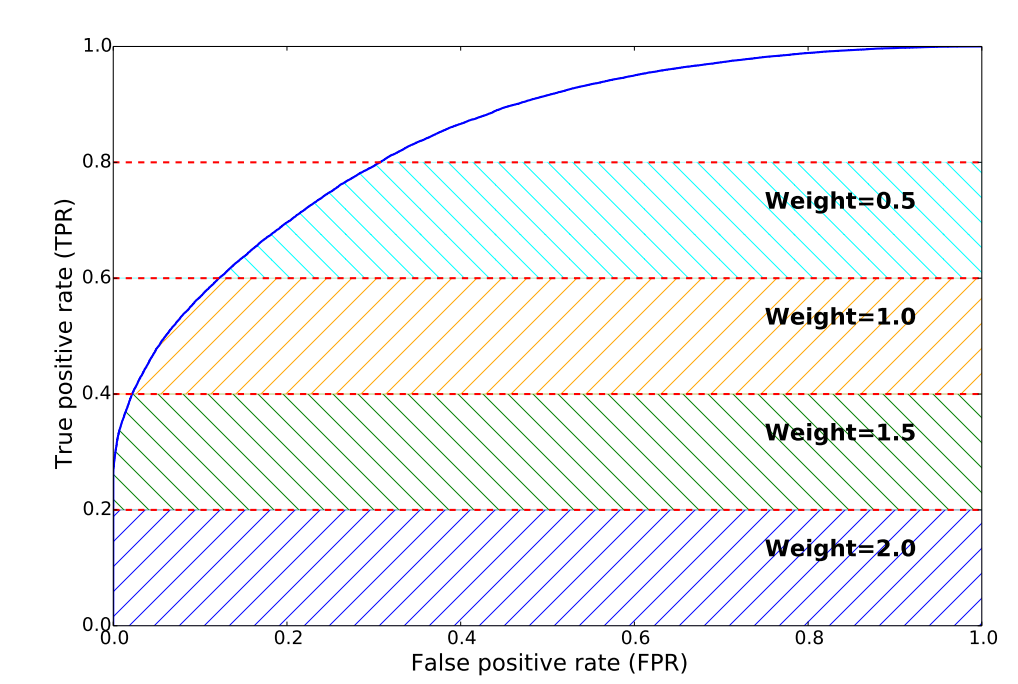
\includegraphics[scale=0.8]{auc.png}
\end{center}


%-------------------------------------------------------
% Применение метода к задаче
\newpage
\section{Применение метода к задаче}
\label{paragraph:architecture}

Далее приведена исследованная нейросетевая архитектура: ее диаграмма, ее описание в виде программного кода на языке Python с использованием фреймворка Keras, а так же описаны методы оценки результатов экспериментов.

\subsection{Описание использованной нейросетевой архитектуры}

Для исследования метода было выбрано следующее строение: % TODO приложить картинку с наглядным описанием


Обучение происходит следующим образом.
Сначала нейросеть обучается при $\lambda = 0$ некоторое количество времени. После этого частично обученная сеть дает результат для данных соответствия, а затем дообучивается с их добавлением следующим образом: на вход классификатору домена для данных соотвествия выставляется метка, получанная ранее, а классификатору домена такая, которая уже находится в данных. Таким образом мы стараемся максимально сохранить результат именно классификатора класса, пытаясь изменить веса внутри экстрактора признаков. При этом мы плавно начинаем повышать $lambda$, каждый раз вычисляя метрики. Останавливаемся в тот момент, когда метрика KS не станет удовлетворять условиям соревнования, а именно станет меньше $0.09$. 

\subsection{Особенности программной реализации}
Для решения задачи был выбран язык программирования Python, а так же фреймворк для проектирования нейронных сетей Keras. Выбор этих инструментов мотивирован простотой их использования.

Отметим отдельно особенности фреймворка Keras, позволяющие лучше описать нейросетевую модель. В версии 1.0.0 во фреймворке появилась так называемое Functional API. Продемонстрируем его применение:

\begin{minted}[fontsize=\small]{python}

n_extracted_features = 100
lam = 0.2

f = feature_extractor(input.shape[1], n_extracted_features)
l = label_classifier(n_extracted_features)
d = label_classifier(n_extracted_features,
                     name="domain_classifier")
	                     
model_input = Input(shape=(f[1],))
features = f(model_input)
label_class = l(features)
grl = GradientReversal(lam, 
                input_shape=(domain_classifier.input_shape[1],))
domain_class = d(grl(f))
m = Model(input=[model_input], output=[label_class, domain_class])
m.compile(loss=['categorical_crossentropy',
   'categorical_crossentropy'], loss_weights=[1, 1],
   metrics=['accuracy', 'accuracy'], optimizer='rmsprop') 
\end{minted}

Как можно заметить, вместо описывания в коде всей нейросети графом, расписывая всех слоев и всех связей между ними, достаточно передать каждому следующему слою предыдущий как аргумент функции. Это заметно упрощает описание модели программным кодом.

\subsection{Оценка результатов работы}

Поскольку в условии задачи явно проверяются показатели AUC, KS и CvM, они и были выбраны для исследования во время эксперимента.

Во время процесса обучения производится нахождение этих показателей. После проведения обучения отрисовывается график, на котором видно их поведение.

Основным показателем качества полученной модели был выбран показатель AUC, который высчитывается при загрузке решения на сайт \texttt{kaggle.com}. В соответствии с этим показателем на этой сайте доступен рейтинг участников. Эти результаты для тех решений, которые удовлетворяют проверке на согласованность и корреляцию (указанные в \ref{agreement_metrics} и \ref{mass_metrics}).


%-----------------------------------------
% Результаты эксперимента
\newpage
\section{Результаты эксперимента}
\label{paragraph:results}

Программа, реализующая выбранную модель, запускалась на компьютере Macbook Pro Late 2013 с процессором 2,4 GHz Intel Core i5 и 8 Гб оперативной памяти. Избранные результаты приведены в таблице ниже.

\begin{table}[!htb]
\caption{\sl Параметры, изменявшиеся во время эксперимента. % TODO описать каждый в этом caption
}
\label{table:results_numeric}

\vspace*{5pt}
\tabcolsep=3pt

\centerline{\resizebox{\textwidth}{!}{%
\begin{tabular}{|c|c|c|c|c|c|c|c|c|}
\hline
id & $extracted\_features$ & $epochs$ & $transfering\_ratio$ & $steps$ & $\lambda_{min}$ & $\lambda_{max}$ & $Dropout$ & agreement\_data\\
\hline
1 & 100 & 400 & 0.75 & 50 & 0 & 0.5 & нет & да \\
\hline
2 & 100 & 400 & 0.80 & 50 & 0 & 0.5 & нет & нет \\
\hline
3 & 100 & 400 & 0.75 & 100 & 0 & 0.2 & да & да \\
\hline
4 & 100 & 400 & 0.79 & 50 & 0 & 0.5 & нет & нет \\
\hline
5 & 100 & 400 & 0.79 & 50 & 0 & 0.5 & нет & да \\
\hline
6 & 100 & 400 & 0.75 & 50 & 0 & 0.8 & да & да \\
\hline
7 & 100 & 400 & 0.80 & 1 & 0.4 & 0.4 & нет & да \\
\hline
8 & 100 & 300 & 0.80 & 50 & 0 & 0.3 & нет & нет \\
\hline
9 & 100 & 130 & 0.5 & 5 & 0.1 & 0.5 & да & да \\
\hline
10 & 120 & 130 & 0.5 & 50 & 1 & 5 & да & да \\
\hline
11 & 120 & 130 & 0.36 & 50 & 0.1 & 0.5 & да & да \\
\hline
11 & 120 & 130 & 0.36 & 50 & 1 & 5 & да & да \\
\hline
\end{tabular}
}}
\end{table}


\begin{table}[!htb]
\caption{\sl Графики поведения метрик \ref{agreement_metrics}, \ref{mass_metrics} и \ref{quality_metrics}}
\label{table:results_graphical}

\vspace*{5pt}
\tabcolsep=3pt
\centerline{
\begin{tabular}{|c|c|c|c|}
\hline
id & KS & CvM & AUC \\
\hline
1 & 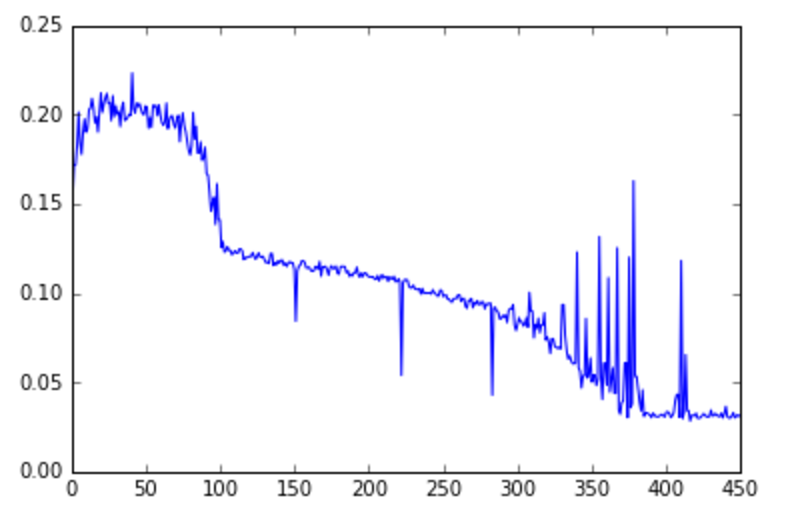
\includegraphics[scale=0.3]{images/ks_1.png} & 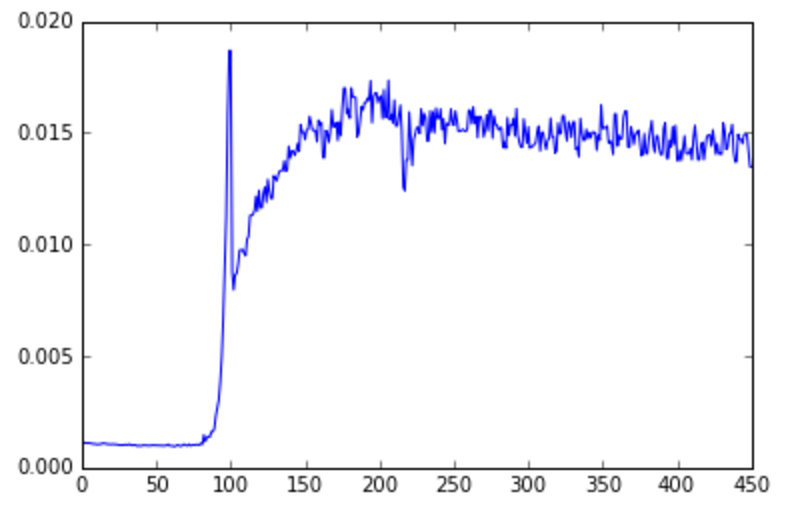
\includegraphics[scale=0.3]{images/cvm_1.png} & 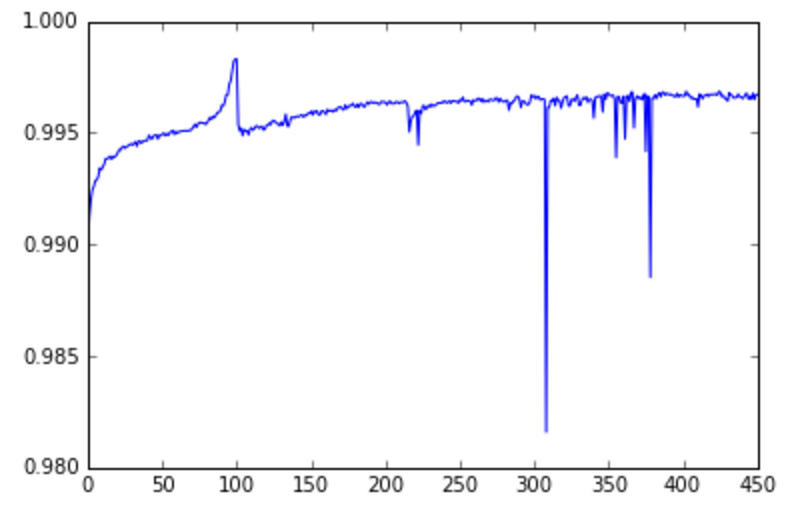
\includegraphics[scale=0.3]{images/auc_1.png} \\
\hline
2 & 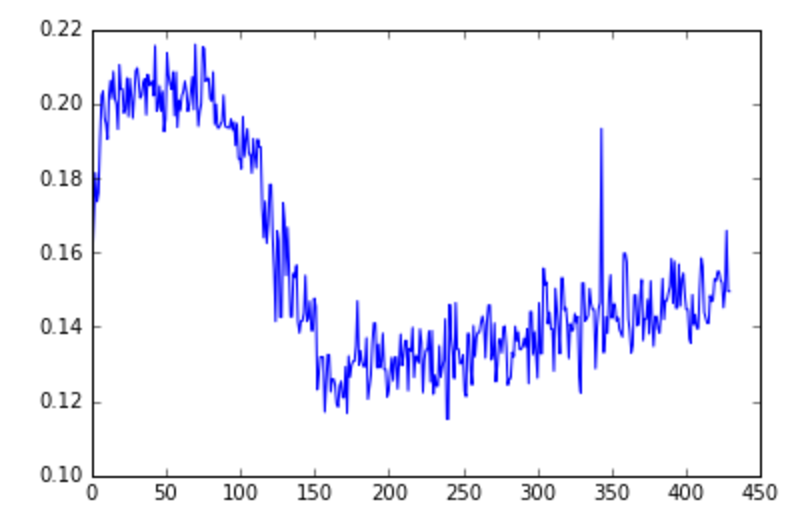
\includegraphics[scale=0.3]{images/ks_2.png} & 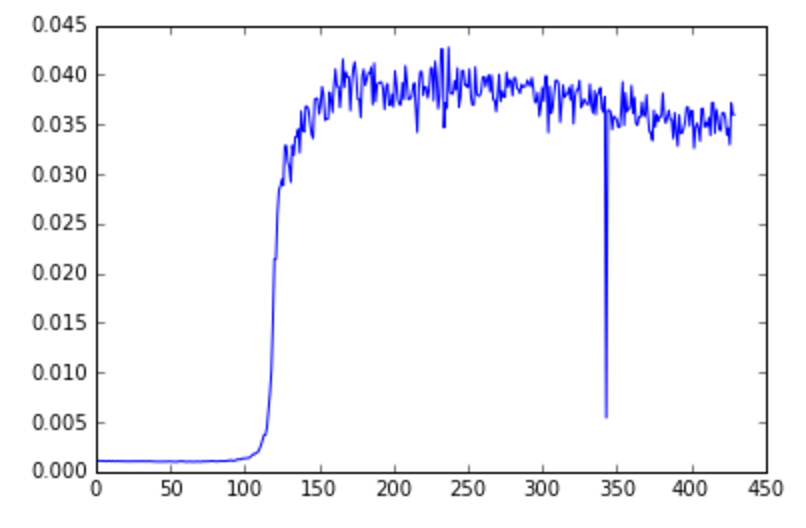
\includegraphics[scale=0.3]{images/cvm_2.png} & 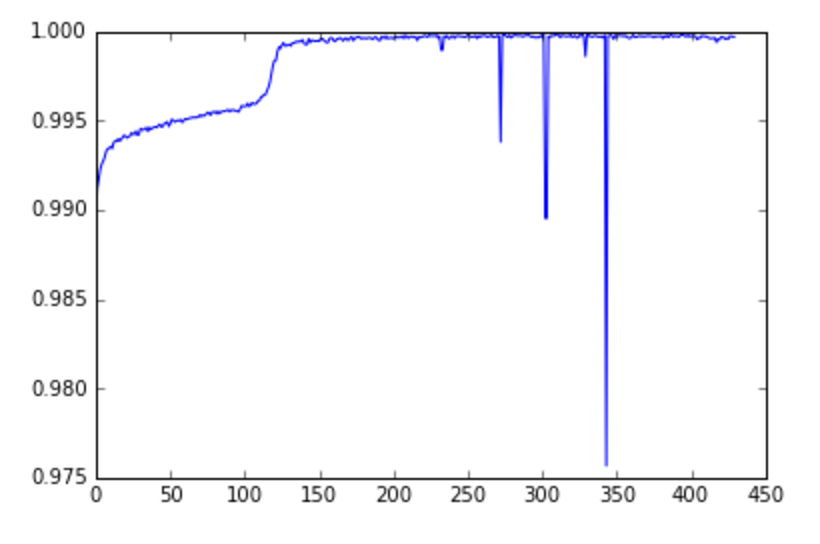
\includegraphics[scale=0.3]{images/auc_2.png} \\
\hline
3 & 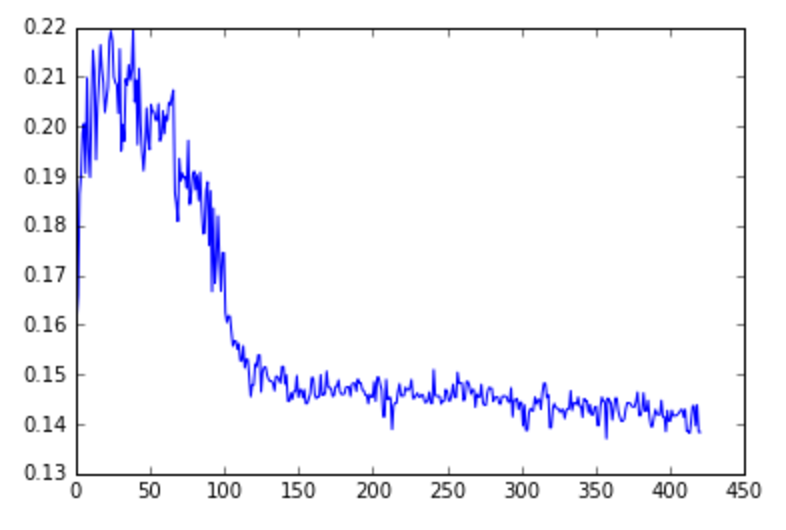
\includegraphics[scale=0.3]{images/ks_3.png} & 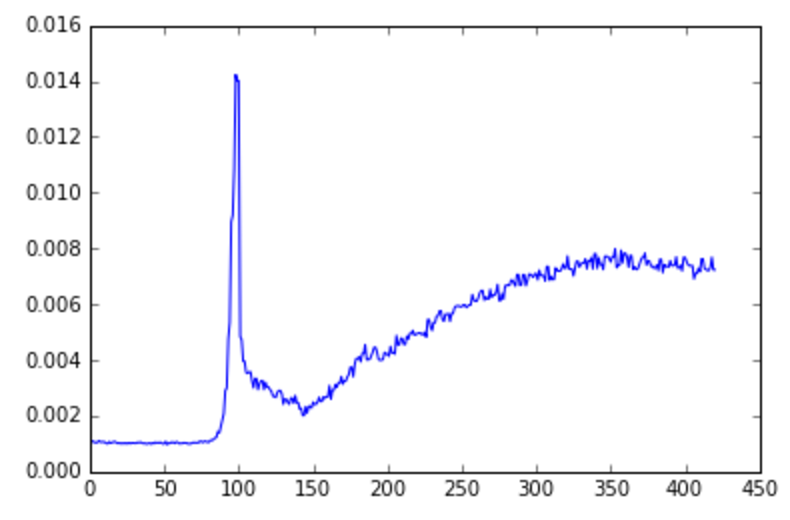
\includegraphics[scale=0.3]{images/cvm_3.png} & 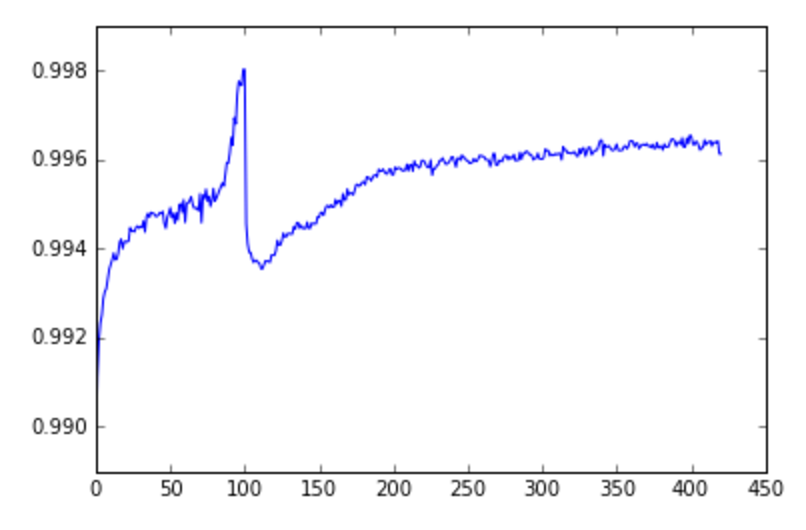
\includegraphics[scale=0.3]{images/auc_3.png} \\
\hline
4 & 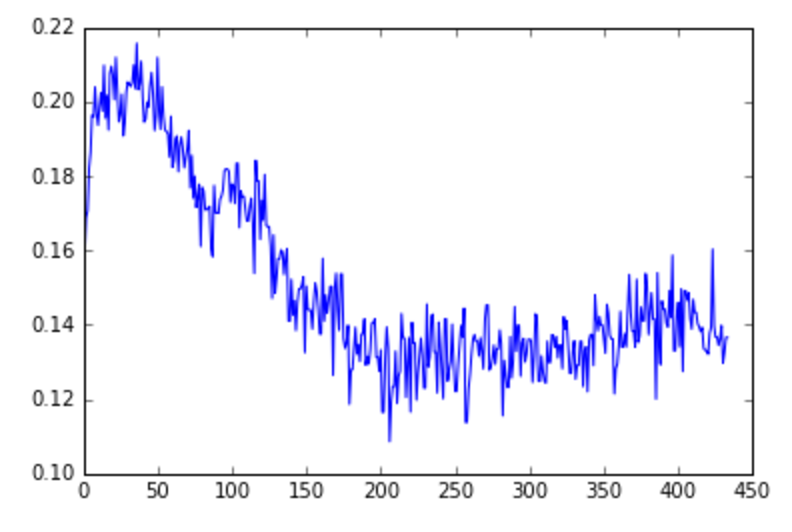
\includegraphics[scale=0.3]{images/ks_4.png} & 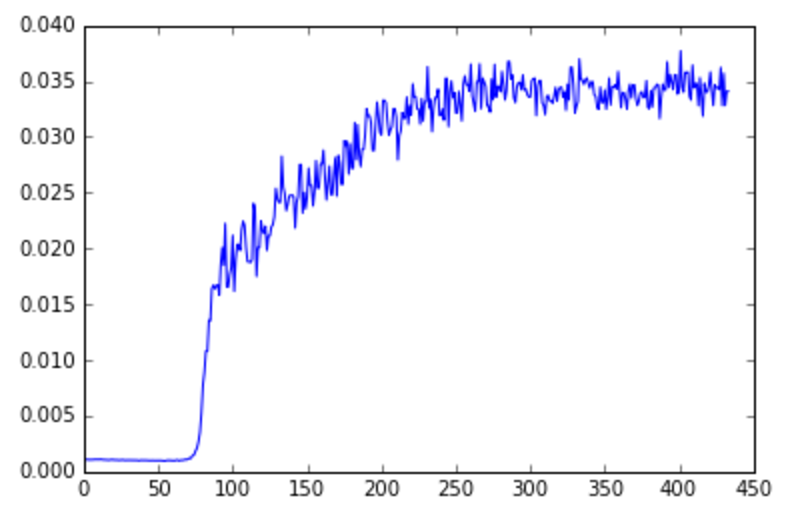
\includegraphics[scale=0.3]{images/cvm_4.png} & 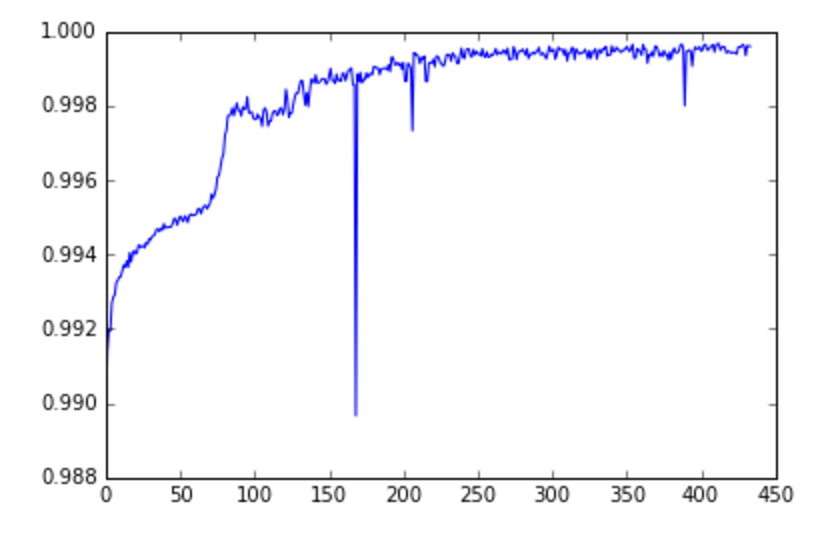
\includegraphics[scale=0.3]{images/auc_4.png} \\
\hline
5 & 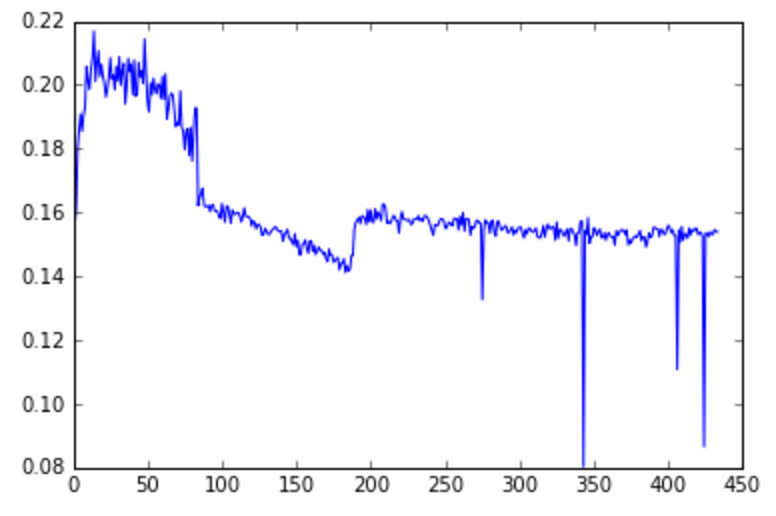
\includegraphics[scale=0.3]{images/ks_5.png} & 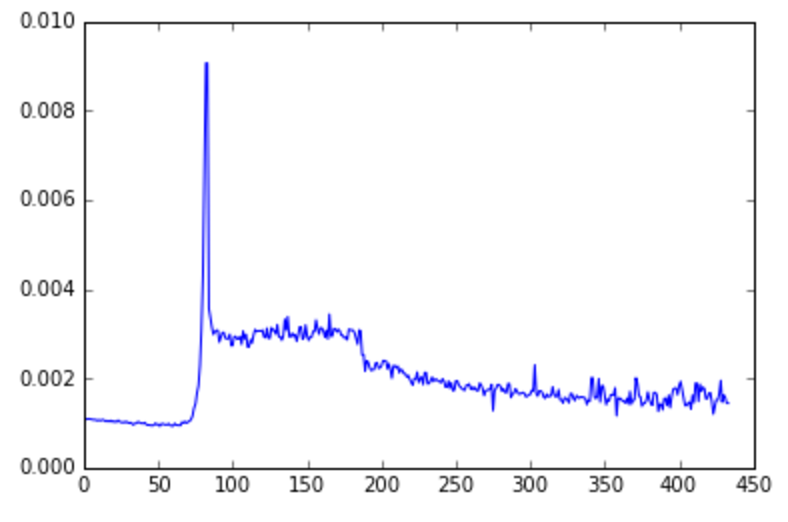
\includegraphics[scale=0.3]{images/cvm_5.png} & 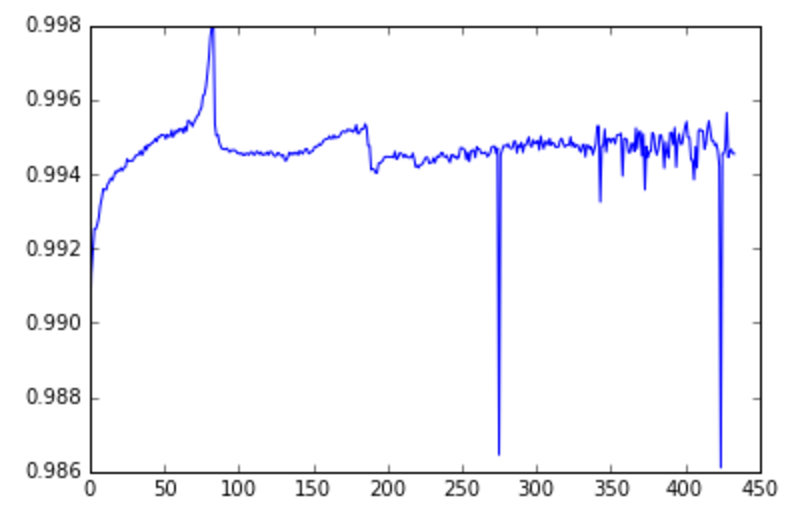
\includegraphics[scale=0.3]{images/auc_5.png} \\
\hline
6 & 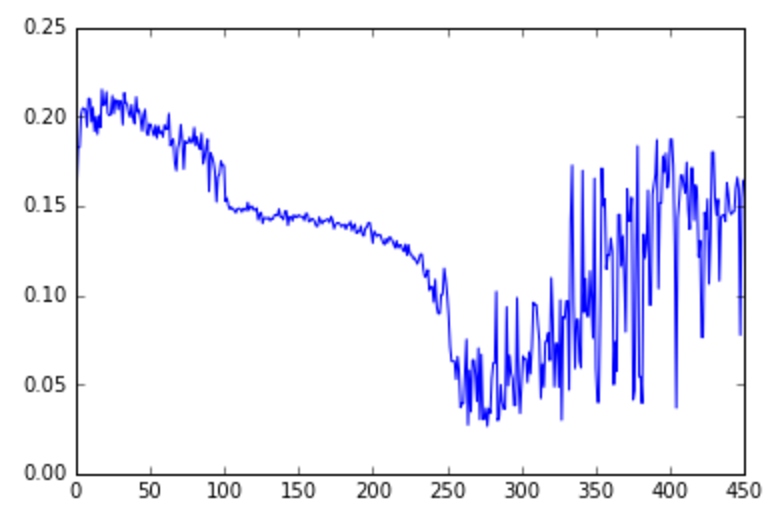
\includegraphics[scale=0.3]{images/ks_6.png} & 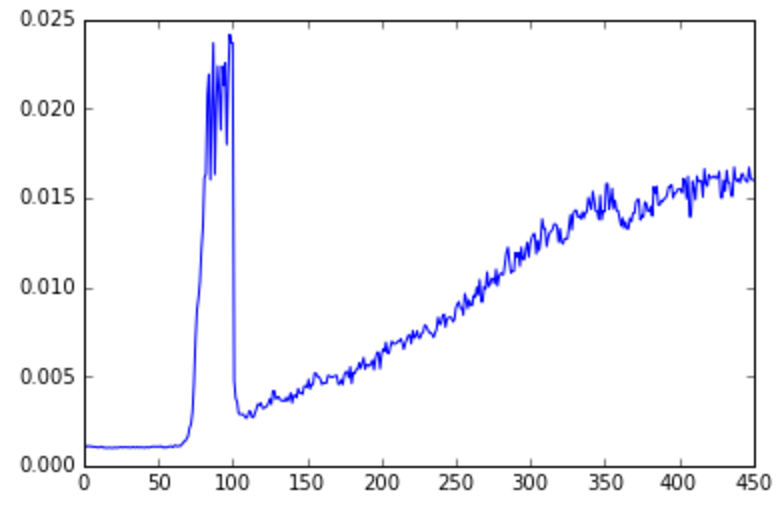
\includegraphics[scale=0.3]{images/cvm_6.png} & 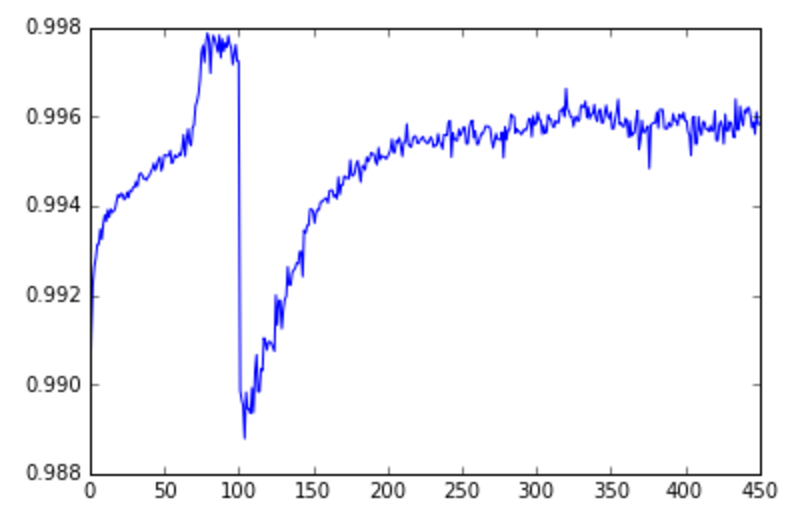
\includegraphics[scale=0.3]{images/auc_6.png} \\
\hline
7 & 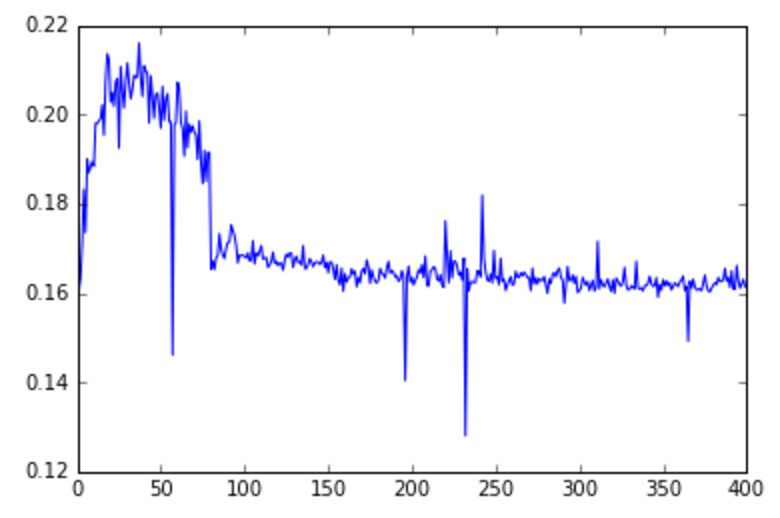
\includegraphics[scale=0.3]{images/ks_7.png} & 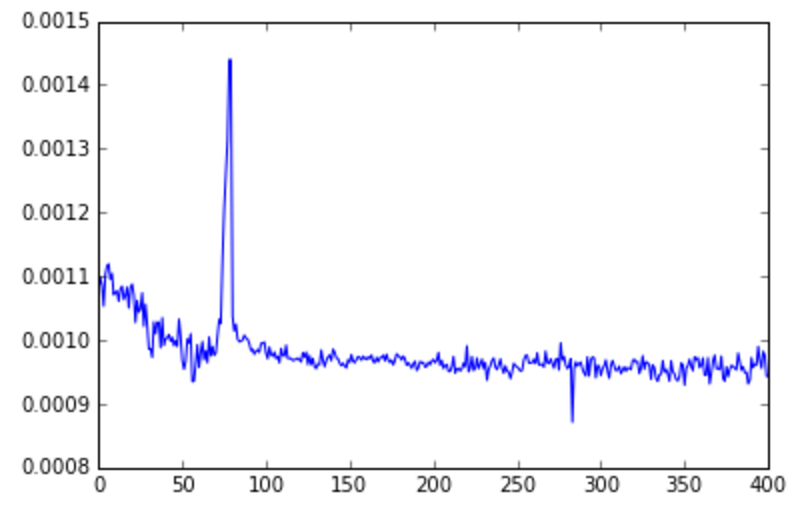
\includegraphics[scale=0.3]{images/cvm_7.png} & 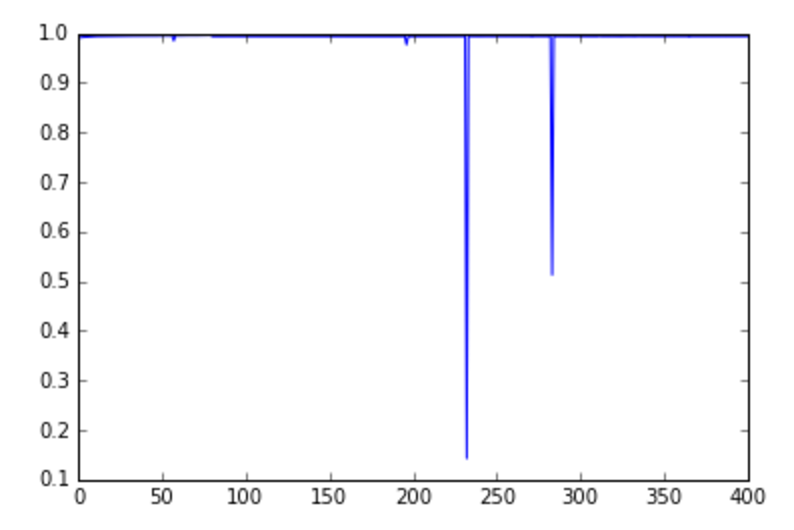
\includegraphics[scale=0.3]{images/auc_7.png} \\
\hline
\end{tabular}
}
\end{table}

\newpage
\begin{table*}[!htb]
\vspace*{5pt}
\tabcolsep=3pt
\centerline{
\begin{tabular}{|c|c|c|c|}
\hline
id & KS & CvM & AUC \\
\hline
8 & 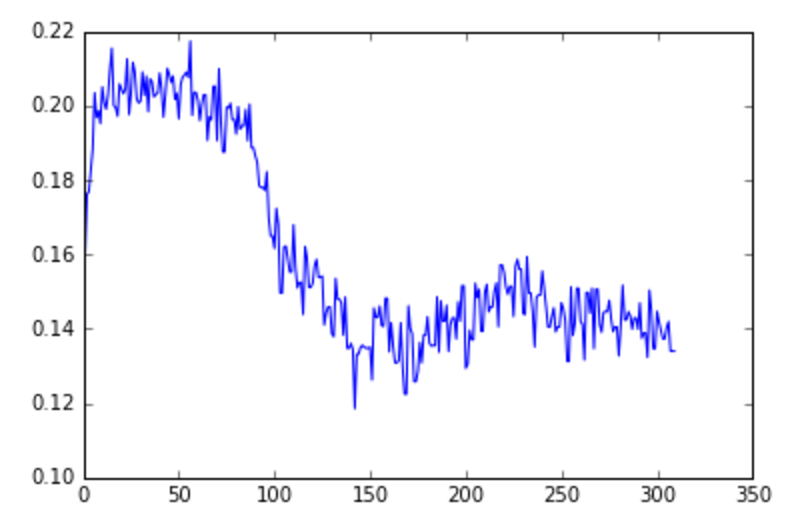
\includegraphics[scale=0.3]{images/ks_8.png} & 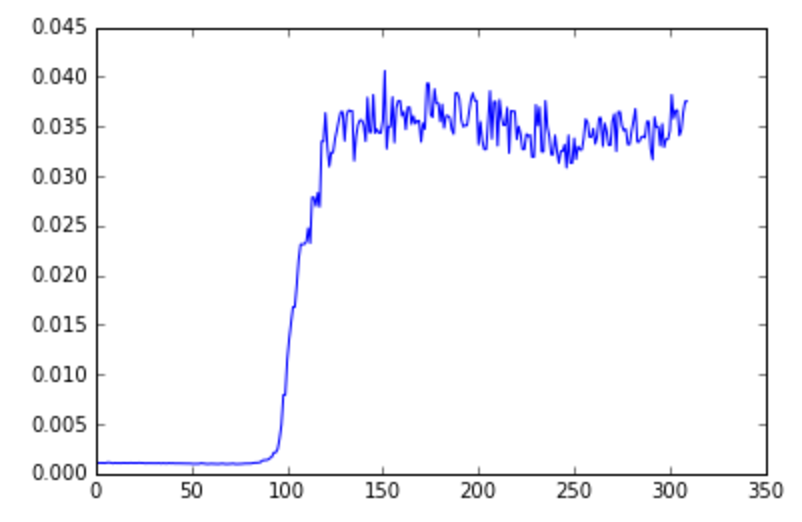
\includegraphics[scale=0.3]{images/cvm_8.png} & 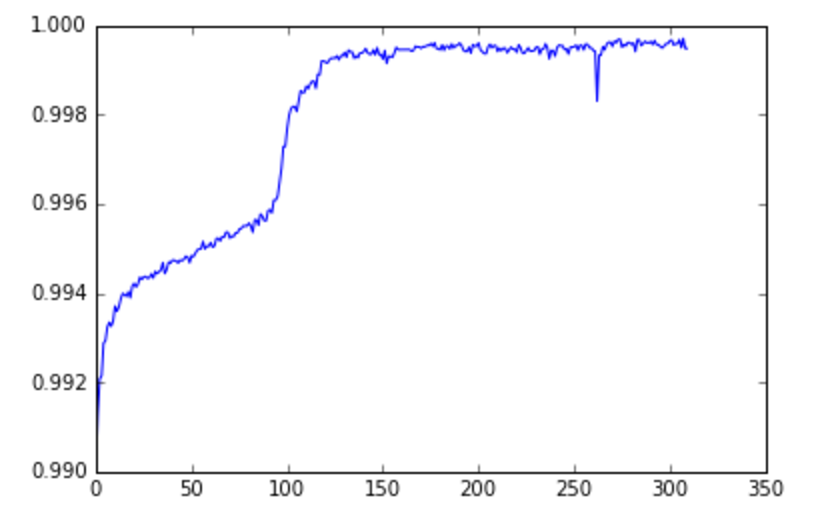
\includegraphics[scale=0.3]{images/auc_8.png} \\
\hline
9 & 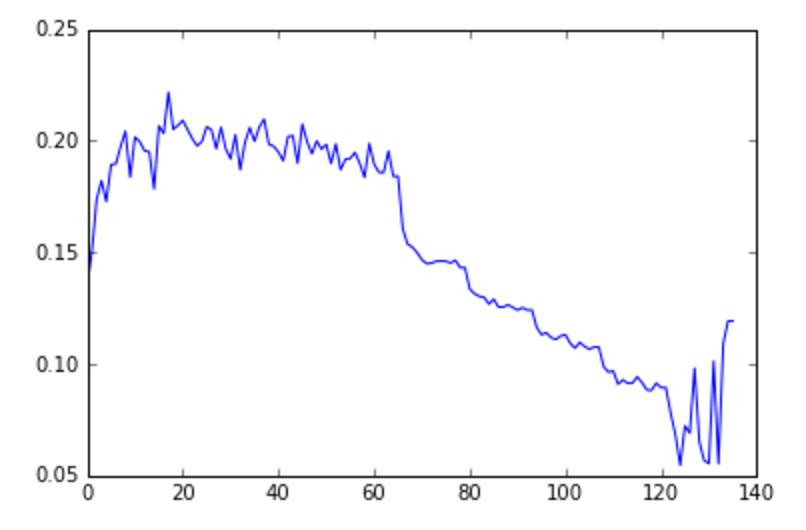
\includegraphics[scale=0.3]{images/ks_9.png} & 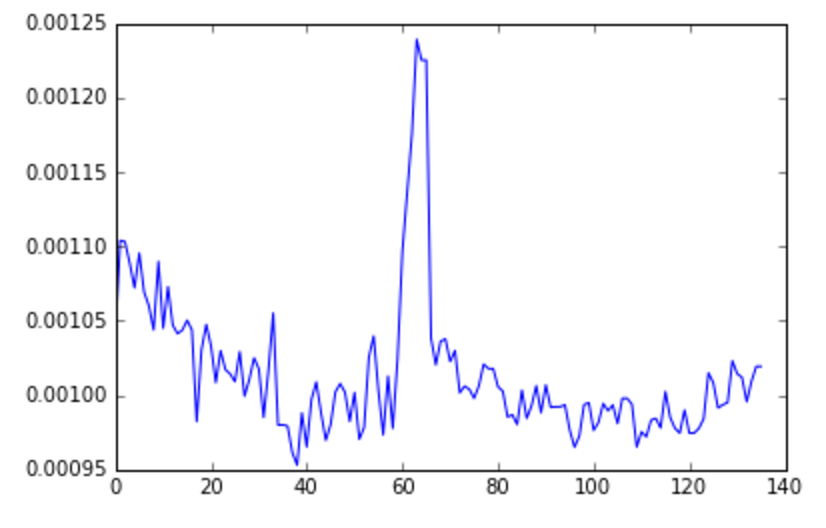
\includegraphics[scale=0.3]{images/cvm_9.png} & 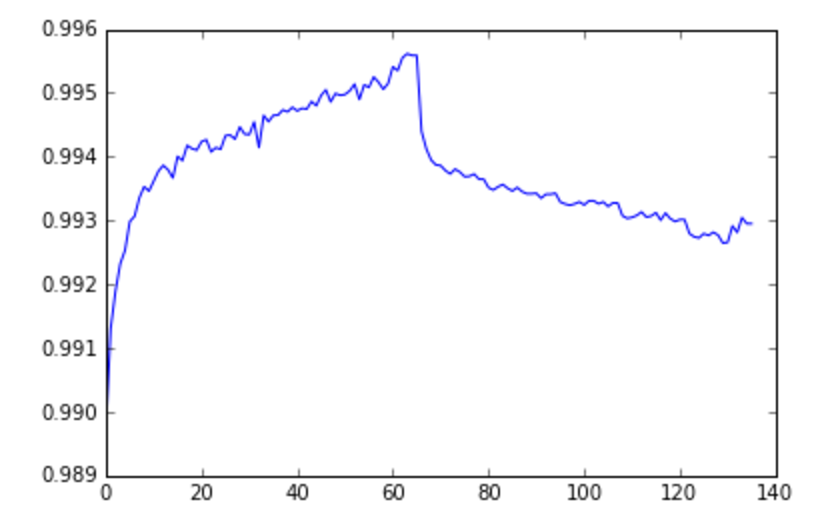
\includegraphics[scale=0.3]{images/auc_9.png} \\
\hline
10 & 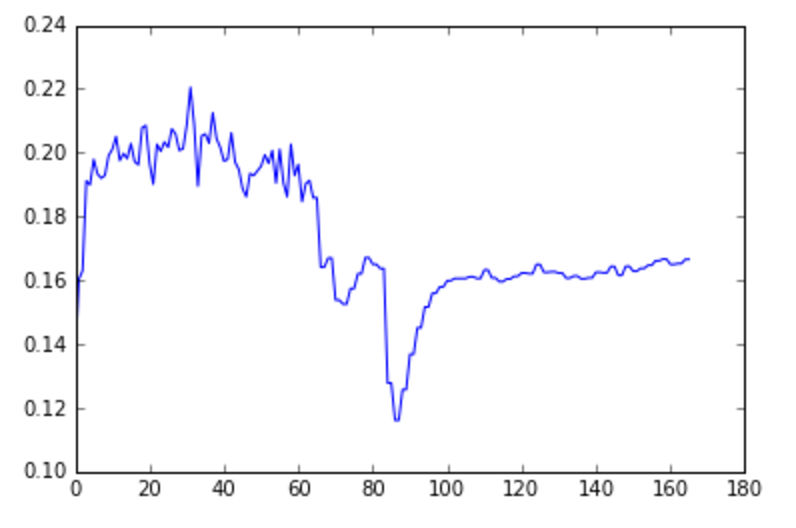
\includegraphics[scale=0.3]{images/ks_10.png} & 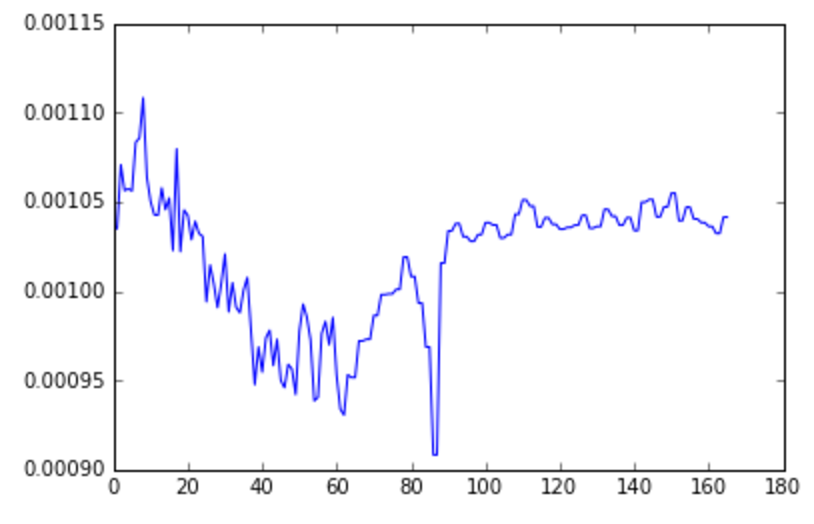
\includegraphics[scale=0.3]{images/cvm_10.png} & 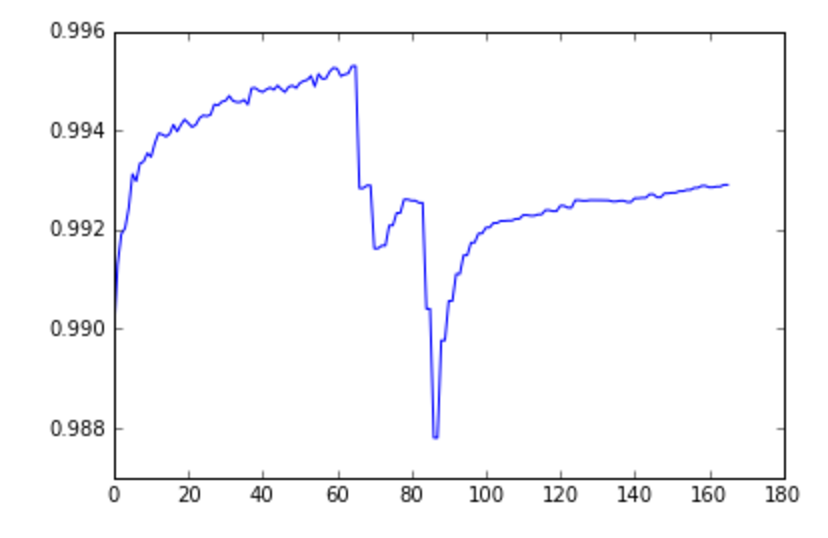
\includegraphics[scale=0.3]{images/auc_10.png} \\
\hline
11 & 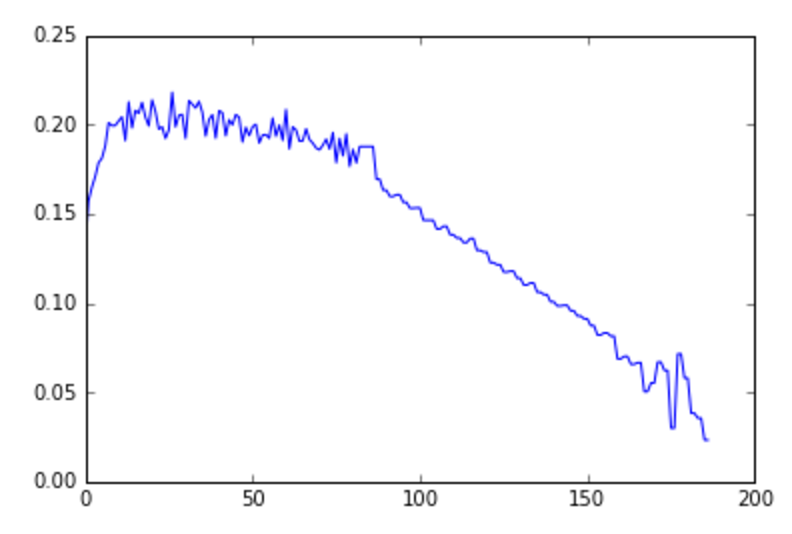
\includegraphics[scale=0.3]{images/ks_11.png} & 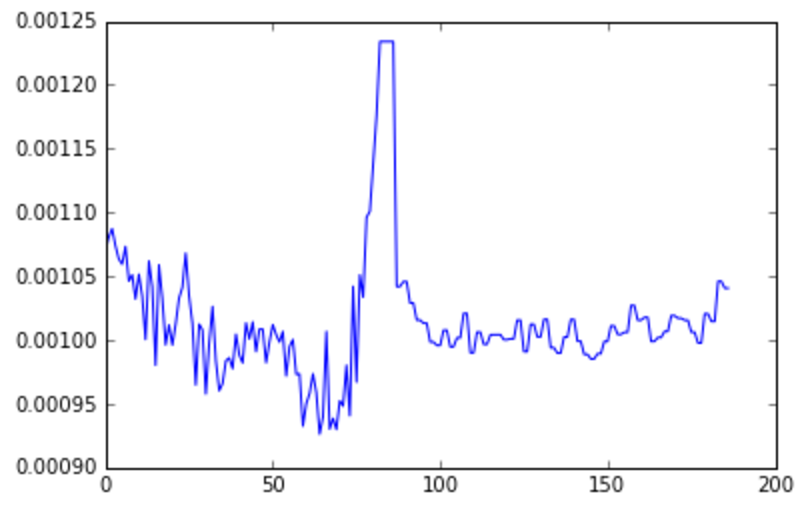
\includegraphics[scale=0.3]{images/cvm_11.png} & 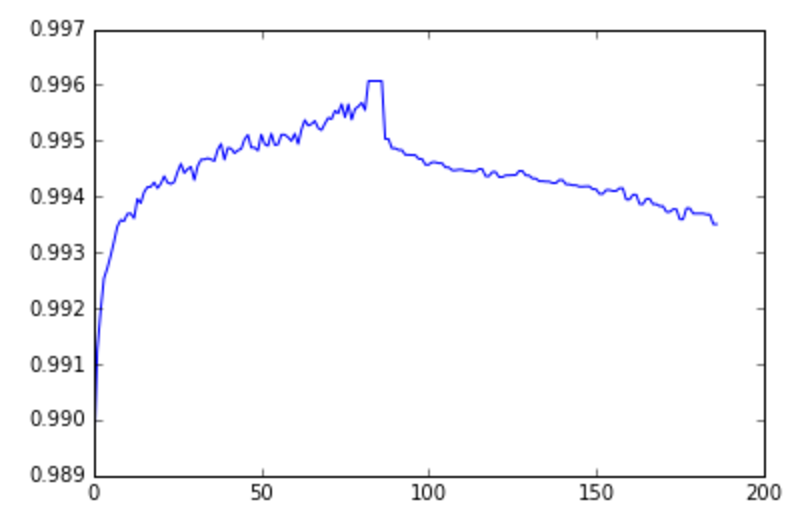
\includegraphics[scale=0.3]{images/auc_11.png} \\
\hline
12 & 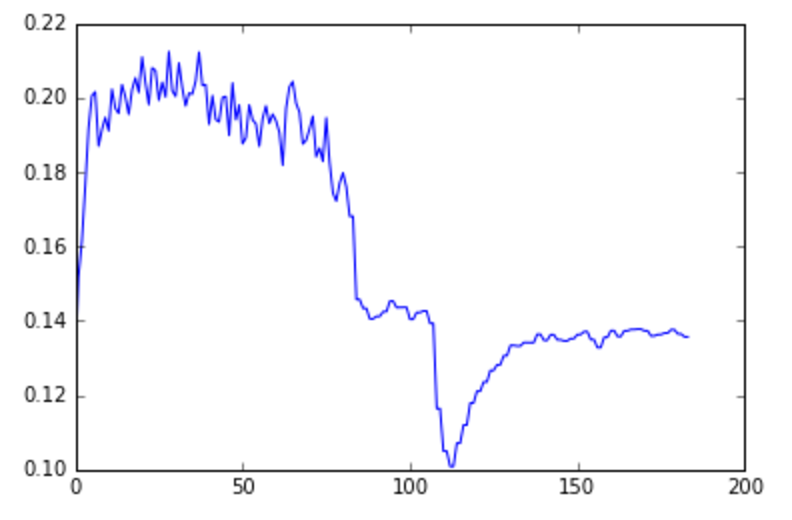
\includegraphics[scale=0.3]{images/ks_12.png} & 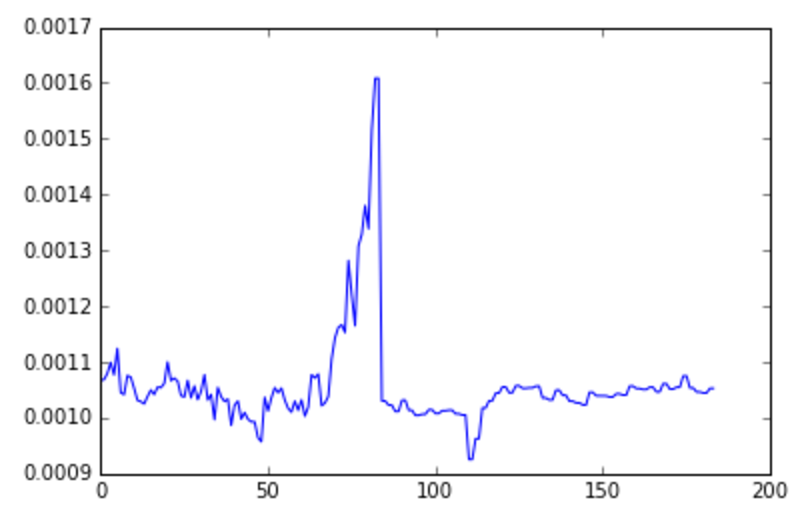
\includegraphics[scale=0.3]{images/cvm_12.png} & 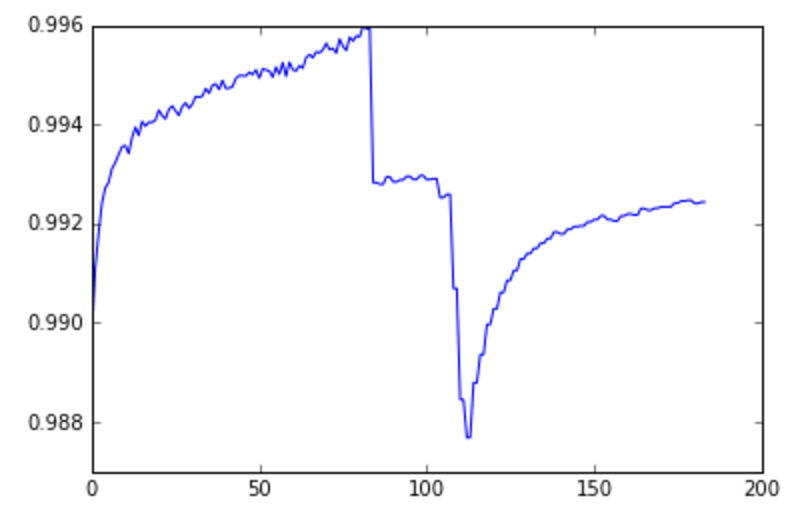
\includegraphics[scale=0.3]{images/auc_12.png} \\
\hline
\end{tabular}
}
\end{table*}

Отметим основные факты, полученные из приведенных выше экспериментов:
\begin{itemize}
	\item После проведения некоторого числа (зависящего от наличия и величины dropout) эпох нейронная сеть начинает коррелировать с массой — другими словами, она формирует признак, который частично ее восстанавливает из исходных данных. Помимо этого, уменьшению параметра CvM после первоначального обучения способствует лишь только использование данных из проверки на соответствие.
	\item Без использования agreement\_data метрика KS занижается, однако недостаточно сильно для засчитывания решения.
\end{itemize}

Таким образом, можно обобщить приведенные выше факты и отметить работоспособность данного метода в этой задаче. Однако, его все еще возможно улучшить. Например, можно на полученных в результате обучения этой нейросетевой модели признаках протестировать другие методы машинного обучения, вроде градиентного бустинга. Помимо этого, имеет смысл получить больше синтетических данных похожей структуры, но другого распада — это может улучшить выделение признаков. Помимо этого, метод стоит попробовать в других задачах — например, в задаче классификации изображений.

%-----------------------------------------
% Заключение
\newpage
\section*{Заключение}
\addtocontents{toc}{\protect{\contentsline{section}{\numberline{}{Заключение}}{\thepage}}}

В работе продемонстрировано применение доменной адаптации в задаче фильтрации событий для детектора частиц коллаборации LHCb Большого Адронного Коллайдера. Были рассмотрены различные приемы обучения нейросетевого классификатора. В результате было получено решение задачи Flavours of Physics на сайте Kaggle, показывающее результат лучше методов, используемых в ЦЕРН. 

Полученную нейронную сеть возможно с легкостью адаптировать для решения других задач.
% TODO подробней


%-----------------------------------------
% Литература
\newpage
\addtocontents{toc}{\protect{\contentsline{section}{\numberline{}{Список литературы}}{\thepage}}}

\begin{thebibliography}{3}  

\bibitem{ganin}
\textit{Yaroslav Ganin, Victor Lempitsky.} Unsupervised Domain Adaptation by Backpropagation \\ \verb|http://arxiv.org/pdf/1409.7495.pdf|

\bibitem{keras}
\textit{François Chollet.} keras, репозиторий GitHub \\ \verb|https://github.com/fchollet/keras|

\bibitem{kaggle}
\textit{Thomas Blake, Marc-Olivier Bettler, Marcin Chrząszcz, Francesco Dettori, Andrey Ustyuzhanin, Tatiana Likhomanenko.} Flavours of Physics: the machine learning challenge for the search of $\tau^-\rightarrow\mu^+ \mu^- \mu^-$ decays at LHCb \\ 
	\verb|https://kaggle2.blob.core.windows.net/competitions/kaggle/|\\ \verb|4488/media/lhcb_description_official.pdf|
	
	
\bibitem{kaggle_contest}
 Flavours of Physics: Finding $\tau^-\rightarrow\mu^+ \mu^- \mu^-$ \\ \verb|https://www.kaggle.com/c/flavours-of-physics/|

\bibitem{cramer}
H. Cram\'er. On the composition of elementary errors — Scandinavian Actuarial Journal, 1928 % http://www.tandfonline.com/doi/pdf/10.1080/03461238.1928.10416862

\bibitem{sgd}
Alex Minnaar. Deep Learning Basics: Neural Networks, Backpropagation and Stochastic Gradient Descent \\
\verb|URL: http://alexminnaar.com/deep-learning-basics-neural-networks-backpropagation-and-stochastic-gradient-descent.html|

\bibitem{dropout}
Nitish Srivastava, Geoffrey Hinton, Alex Krizhevsky, Ilya Sutskever, Ruslan Salakhutdinov. Dropout: A Simple Way to Prevent Neural Networks from
Overfitting. \\ \verb|URL: https://www.cs.toronto.edu/~hinton/absps/JMLRdropout.pdf|

\bibitem{prelu}
Kaiming He, Xiangyu Zhang, Shaoqing Ren, Jian Sun. Delving Deep into Rectifiers:
Surpassing Human-Level Performance on ImageNet Classification. \\\verb|URL: https://arxiv.org/pdf/1502.01852v1.pdf|

\end{thebibliography}

\label{page:last}

\end{document}
